%%%%%%%%%%%%%%%%%%%%%%%%%%%%%%%%%%%%%%%%%%%%%%%%%%%%%%%%%%%%%%%%%%%%%%
% Overleaf (WriteLaTeX) Example: Molecular Chemistry Presentation
%
% Source: http://www.overleaf.com
%
% In these slides we show how Overleaf can be used with standard 
% chemistry packages to easily create professional presentations.
% 
% Feel free to distribute this example, but please keep the referral
% to overleaf.com
% 
%%%%%%%%%%%%%%%%%%%%%%%%%%%%%%%%%%%%%%%%%%%%%%%%%%%%%%%%%%%%%%%%%%%%%%
% How to use Overleaf: 
%
% You edit the source code here on the left, and the preview on the
% right shows you the result within a few seconds.
%
% Bookmark this page and share the URL with your co-authors. They can
% edit at the same time!
%
% You can upload figures, bibliographies, custom classes and
% styles using the files menu.
%
% If you're new to LaTeX, the wikibook is a great place to start:
% http://en.wikibooks.org/wiki/LaTeX
%
%%%%%%%%%%%%%%%%%%%%%%%%%%%%%%%%%%%%%%%%%%%%%%%%%%%%%%%%%%%%%%%%%%%%%%

\documentclass{beamer}
\usepackage{graphicx}
\graphicspath{ {images/} }
% For more themes, color themes and font themes, see:
% http://deic.uab.es/~iblanes/beamer_gallery/index_by_theme.html
%
\mode<presentation>
{
  \usetheme{Madrid}       % or try default, Darmstadt, Warsaw, ...
  \usecolortheme{default} % or try albatross, beaver, crane, ...
  \usefonttheme{serif}    % or try default, structurebold, ...
  \setbeamertemplate{navigation symbols}{}
  \setbeamertemplate{caption}[numbered]
} 

\usepackage[english]{babel}
\usepackage[utf8x]{inputenc}
\usepackage{chemfig}
\usepackage[version=3]{mhchem}

% On Overleaf, these lines give you sharper preview images.
% You might want to `comment them out before you export, though.
\usepackage{pgfpages}
\pgfpagesuselayout{resize to}[%
  physical paper width=8in, physical paper height=6in]

% Here's where the presentation starts, with the info for the title slide
\title[Molecules in \LaTeX{}]{Identifying, Recognition, and Diagnosing Students with Learning Disabilities and Depression Based on Artificial Intelligence}
\author{Do Dung Vu}
\institute{Supervised by: Prof. Sylvie Ratté}
\date{\today}

\begin{document}

\begin{frame}
  \titlepage
\end{frame}

% These three lines create an automatically generated table of contents.
\begin{frame}{Outline}
  \tableofcontents
\end{frame}

\section{Introduction}
\subsection{Statistics of Disability and Depression}
\begin{frame}{Introduction}

\frametitle{Statistics of Disability and Depression}

\begin{columns}
		\begin{column}{0.5\textwidth}  %%<--- here
		\begin{center}
			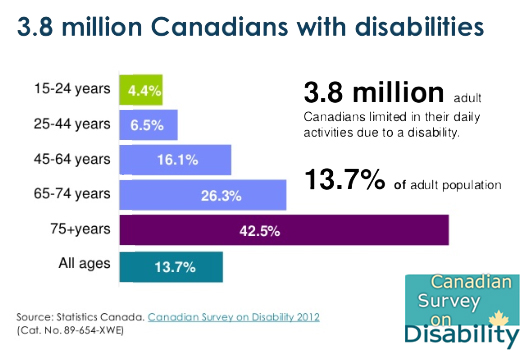
\includegraphics[width=1\textwidth]{CanadianSurveyOfDisability.jpg}
		\end{center}
		{\tiny 	Source: https://www.technologyreview.com}
	\end{column}
	\begin{column}{0.5\textwidth}
		\begin{itemize}
			\item 	Almost 14 percent of the Canadian population aged 15 years or older – or 3.8 million individuals – reported a difficulty or impairment due to a long-term condition or health problem that limited their daily activities.
			\item The prevalence of disability increased with age, with the average onset age in early 40s.
			
		\end{itemize}
		
	\end{column}

\end{columns}
\end{frame}

\subsection{Artificial Intelligence in Health Care}
\begin{frame}{Introduction}

\frametitle{Artificial Intelligence in Health Care}

\begin{columns}
	\begin{column}{0.5\textwidth}
		\begin{itemize}
			\item  AI is exploding in popularity.
			\item  Growth in the AI health market is expected to reach 	\textdollar 6.6 billion by 2021—that is a compound annual growth rate of 40\%
			\item E.g.,	Software that can understand images, sounds, and language is being used to help people with disabilities and depression such as deafness and autism in new ways.
		\end{itemize}

	\end{column}
	\begin{column}{0.5\textwidth}  %%<--- here
		\begin{center}
			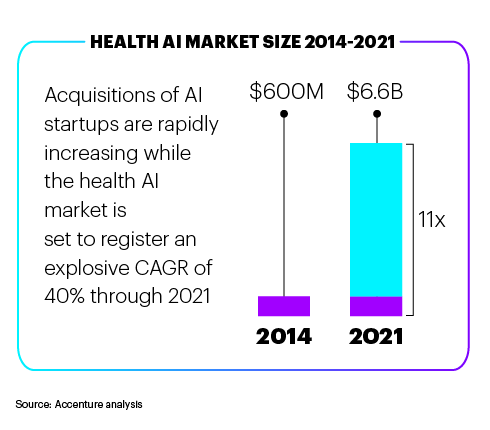
\includegraphics[width=0.7\textwidth]{AI.png}
		\end{center}
		\begin{center}
		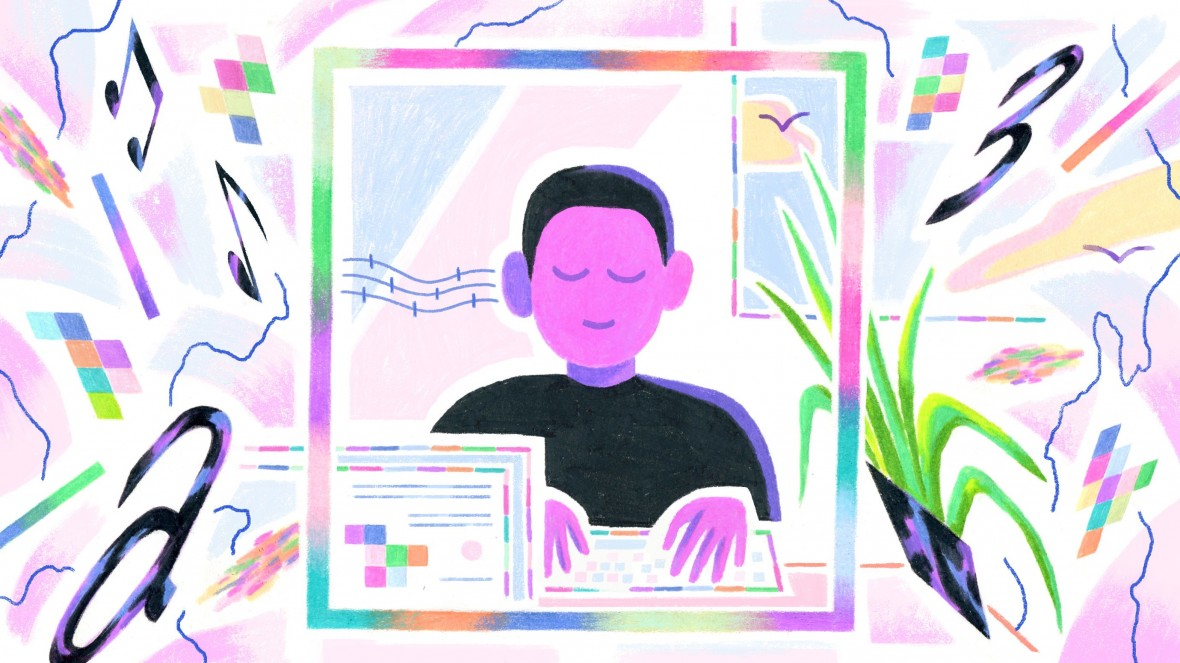
\includegraphics[width=0.7\textwidth]{MLL.jpg}
	\end{center}
{\tiny 	Source: https://www.technologyreview.com}
	\end{column}
\end{columns}
\end{frame}

\section{Problem}

\subsection{Problem}
\begin{frame}{Problem}
\begin{columns}
	\begin{column}{0.5\textwidth}  %%<--- here
		\begin{center}
			
\includegraphics[width=1\textwidth]{Learn.jpg}
		\end{center}
		{\tiny 	Source: https://www.vamosblog.co.uk}
	\end{column}
	\begin{column}{0.5\textwidth}
		\begin{itemize}
			\item How to identify, recognize, and diagnosing students with learning disabilities and depression.
			\item How to recommend the insightful and effective therapy to solve these issues.
			
		\end{itemize}
		
	\end{column}
	
\end{columns}

\end{frame}

\section{Literature Survey}

\subsection{Literature Review}
\begin{frame}{Literature Review}
\begin{itemize}
	\item A system that can recognize such kind of actions
	using deep learning techniques thereby, notifying the
	caretakers/parents so that they can get the situation under control
	in lesser time \cite{Venkata}
	\item A deep neural network architecture
	to address the Facial Expression Recognition problem across multiple wellknown standard face datasets \cite{Mollahosseini}. Moreover, a Mobile Face Recognition System for
	Visually Impaired Persons is proposed in \cite{Chaudhry}
	\item Enhancing deep learning sentiment analysis with ensemble techniques in social applications which can be utilized to detect and prevent the depression \cite{Araque}
	\item Down Syndrome Prediction/Screening Model Based on Deep Learning and Illumina
	Genotyping Array is proposed in \cite{Feng}
\end{itemize}

\end{frame}
\subsection{Reference}

\begin{frame}{Reference}
 \begin{thebibliography}{99}
	\bibitem{Venkata}{\tiny  V. S. P. Patnam, F. T. George, K. George and A. Verma, "Deep Learning Based Recognition of Meltdown in Autistic Kids," 2017 IEEE International Conference on Healthcare Informatics (ICHI), Park City, UT, 2017, pp. 391--396 
}
	
		\bibitem{Mollahosseini}{\tiny A. Mollahosseini, D. Chan and M. H. Mahoor, "Going deeper in facial expression recognition using deep neural networks," 2016 IEEE Winter Conference on Applications of Computer Vision (WACV), Lake Placid, NY, 2016, pp. 1--10}
		\bibitem{Chaudhry}{\tiny S. Chaudhry and R. Chandra, "Design of a Mobile Face Recognition System for
	Visually Impaired Persons, in arXiv: 1502.00756v2
	\bibitem {Araque}O. Araque, I. C.-Platas, J. Fernando S.-Rada, C. A. Iglesias,
		Enhancing deep learning sentiment analysis with ensemble techniques in social applications,
		Expert Systems with Applications,
		Volume 77,
		2017,
		pp 236--246}
		\bibitem{Feng}{\tiny B. Feng, D. C. Samuels, W. Hoskins, Y. Guo, Y. Zhang, J. Tang, and Z. MEng, ``Down syndrome prediction/screening model based on deep learning and illumina genotyping array," 2017 IEEE International Conference on Bioinformatics and Biomedicine (BIBM), Kansas City, MO, 2017, pp. 347--352}
\end{thebibliography}
\end{frame}
\section{Challenges}


\begin{frame}{Challenges}
\begin{itemize}
	\item Identify and recognize the sentiment and emotion features
	\item Faster handling of responding for real time used cases
	\item Data authenticity, confidentiality, ready, and integrity for real time applications (e.g., social media, crowd sourcing)
	\item The accurately predict what types of catastrophic incidents might put patients back into the hospital
	\item Maintain the patient identity, location, security, and privacy
	
\end{itemize}
\end{frame}
\section{Objectives}


\begin{frame}{Objectives}
\begin{itemize}
	\item Enhance privacy system to Identify, Recognize, and Diagnose Students with Learning Disabilities and Depression 
	\item Improve the accuracy and performance of object recognizing to detect the semantic and behavivor features 
	\item Develop algorithms to analyze the sentiment bahavior of the depression information on the social network
	\item Develop algorithm to evaluate and analyze the progress of depression and diabiliies learning
	
\end{itemize}
\end{frame}
\section{Methodology}


\begin{frame}{Methodology}
\begin{itemize}
	\item Exploit the Artificial, Deep, Recurrent, Convolutional neural networks (ANN,DNN,RNN,CNN), Supervised, Unsupervised, and Deep Reinforcement learning, Search Engine algorithm to improve the quality of object recognition
	\item Apply a natural language user interface to attempt to answer questions, make recommendation
	\item Predict the negative or dangerous behavior of disabilities and depression student based on the social media network
	
\end{itemize}
\end{frame}
\section{Proposed Contribution}

\begin{frame}{Expectation of Contribution}
\begin{itemize}
	
	\item  A privacy system to Identify, Recognize, and Diagnose Students with Learning Disabilities and Depression 
	\item A new solution for Disabilities and Depression Therapy by tracing, evaluating, analyzing both the sentiment of user behavior in the real world and social network
\end{itemize}
\end{frame}
\section{Study Plan}


\begin{frame}{Study Plan}
	\begin{center}
	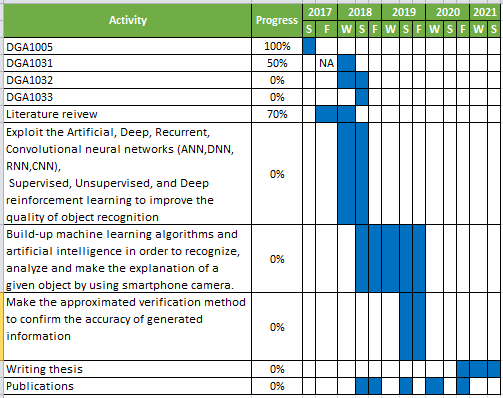
\includegraphics[width=0.8\textwidth]{StudyPlan.png}
\end{center}
\end{frame}
\end{document}